% include the figures path relative to the master file
\graphicspath{{./content/intro/figures/}}
\section{Setting the polarimetric camera for robotics}
\label{sec:rosify}

In this work, visual information is captured using the \emph{IMPREX Bobcat GEV}
polarimetric camera which is a \gls{dofp} polarimetric camera. In a single shot,
the camera captures four different linearly polarized measures by using
a micropolarizer with pixelated polarized filter array as illustrated in
Fig.\,\ref{fig:dofp-sensor}. Hence, each acquired image is subdivided into four
linearly polarized images $I_0$, $I_{45}$, $I_{135}$, and
$I_{90}$. Subsequently, the polarized state of the incident light is computed
from these images by means of the Stokes'
parameters~\cite{goldstein2017polarized}, referred as $s_0$, $s_1$, and $s_2$
in Eq.\,\ref{eq:stokes}. In addition, the polarized parameters \gls{aop} and
\gls{dopl}, respectively referred $\alpha$ and $\rho_l$ in
Eq.\,\ref{eq:stokes}) are computed.

% As mentioned previously, in this work we use a \gls{dofp} polarimetric camera,
% to be exact \textit{IMPREX Bobcat GEV polarimetric camera}.
% This camera has the advantage to capture four different linearly polarized
% measure in one image, due to their micropolarizer and pixelated polarized
% filter array (see Fig.\,\ref{fig:dofp-sensor}).
% Therefore each capture image leads to four linearly polarized sub-image $I_0$,
% $I_{45}$, $I_{135}$, $I_{90}$.
% Using these four measurements, the polarized state of the incident light is
% calculated in terms of stokes parameters~\cite{goldstein2017polarized}, which
% are used thereafter to calculate polarized parameters such as \gls{aop} refered
% as $\alpha$ and \gls{dopl} refered as $\rho_l$ (see Eq.\,\ref{eq:stokes}).

\begin{figure}
  \centering
  \includegraphics[width=0.3\textwidth]{./content/intro/figures/dofp-sensor-0-45-135-90.jpg}
  \caption{Structure of \gls{dofp} sensors: in a single shot, four polarized
    images are acquired, each of them with a different polarized angles.}
    \label{fig:dofp-sensor}
\end{figure}

\begin{figure*}
  \centering
  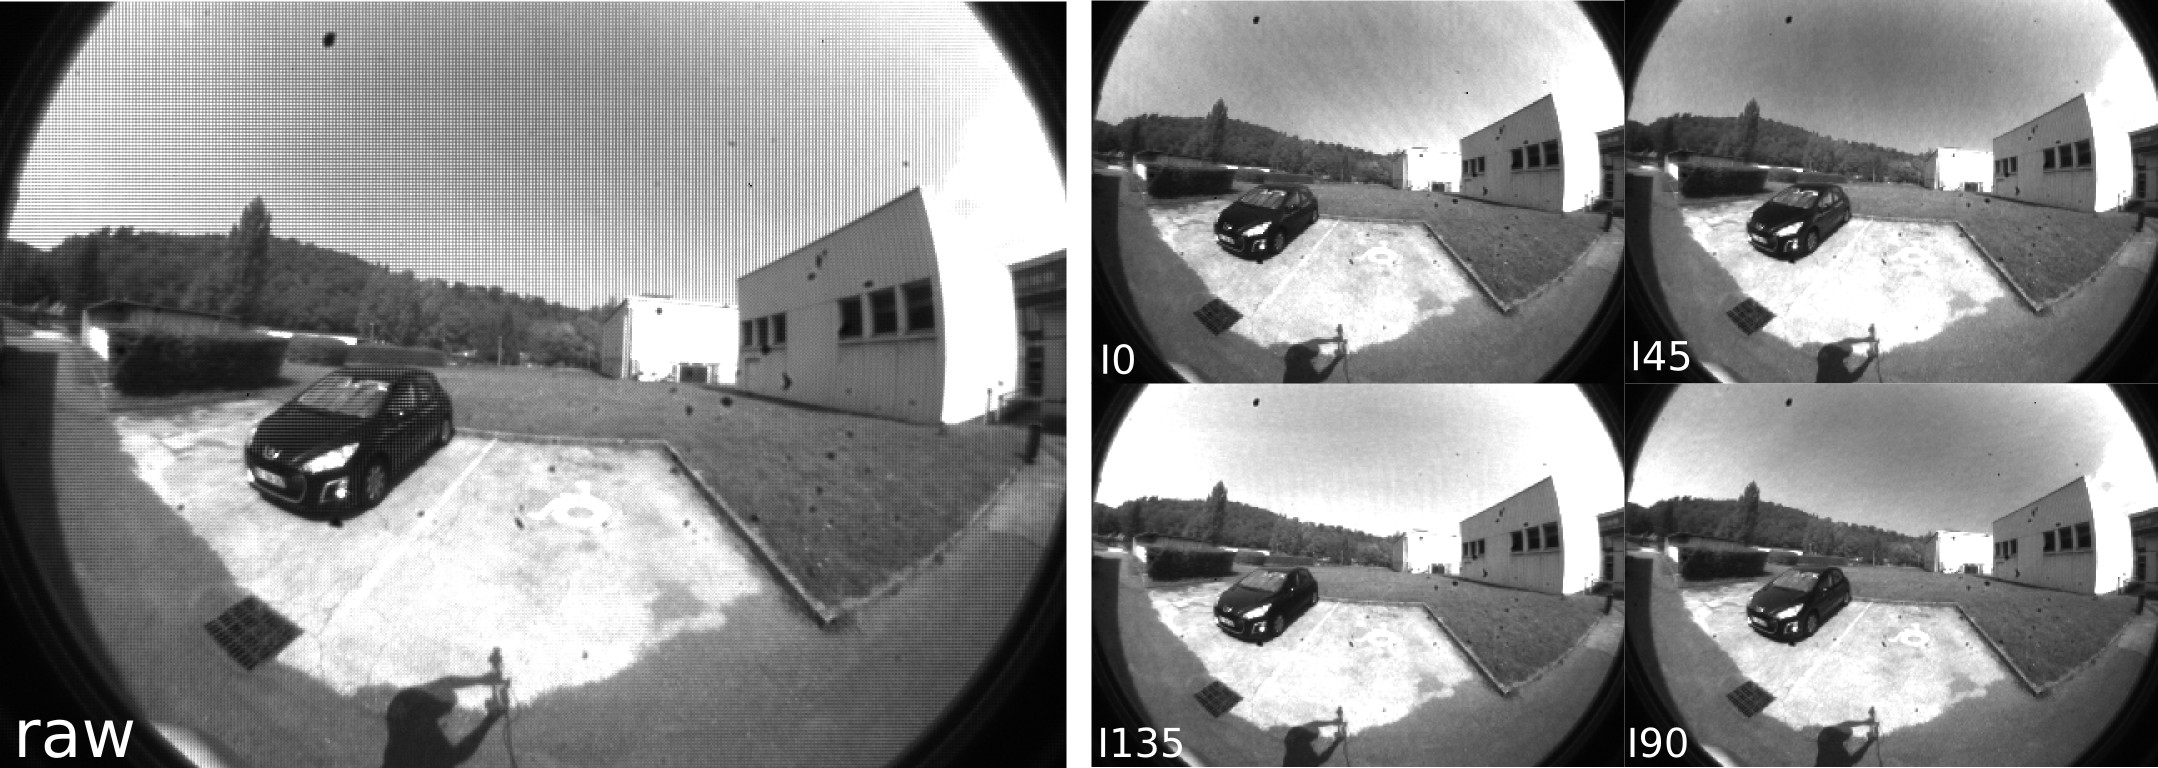
\includegraphics[width=0.7\textwidth]{./content/intro/figures/raw-sp.jpg}
  \caption{A raw image captured with fisheye lens, and the extracted four
    linearly polarized images ($I_0, I_{45}, I_{135}, I_{90}$)}
  \label{fig:raw-sp}
\end{figure*}

\begin{figure}
  \centering
  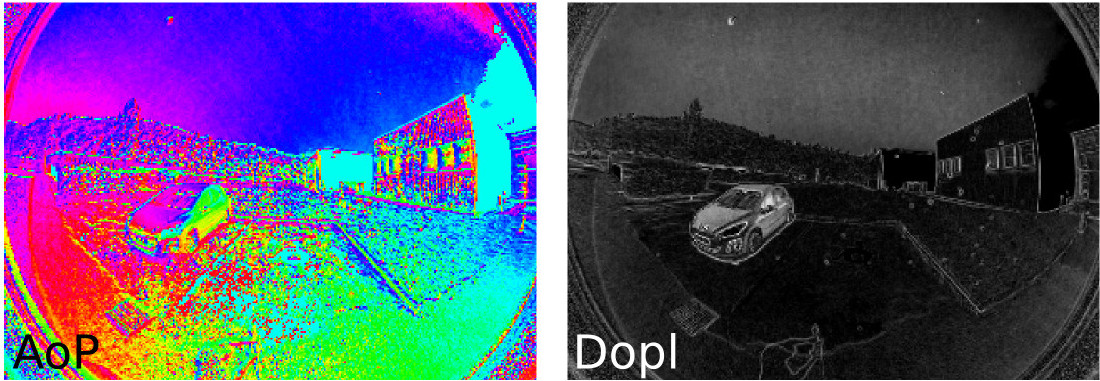
\includegraphics[width=0.47\textwidth]{./content/intro/figures/aop-dop.jpg}
  \caption{The \gls{aop}, and \gls{dopl} images. For visualization purpose,
    \gls{aop} is represented in $hsv$ color space.
    \label{fig:stokes-aop-dop}}
\end{figure}


\begin{gather}
  \begin{aligned}
    % \small
    s_0 & = \frac{I_0 + I_{45} + I_{135} + I_{90}}{4}\\
    s_1 & = I_0 - I_{90} \\
    s_2 & = I_{45} - I_{135} \\
    \alpha &= 0.5 \arctan(\frac{s_2}{s_1}) \\
    \rho_l &= \frac{\sqrt{s_2^{2} + s_1^{2}}}{s_0}
    \label{eq:stokes}
  \end{aligned}
\end{gather}

From the raw images ($640\times460$) captured by the camera, the sub-images can
be extracted directly using super-pixel method that leads to four images, half
of the size of the raw image, or can be interpolated to the full
size~\cite{ratliff2009interpolationmicrogrid,gao2011bilinearpolarimeters}.  The
super-pixel method was used for the results presented in this paper. Being
interested in large-field of view, a fisheye lens of 180-degree was used on the
camera.

An example of captured raw image, the linearly polarized images and polarized
information is shown in Fig.~\ref{fig:raw-sp}~$\&$~\ref{fig:aop-dop}.

The \textit{IMPREX Bobcat GEV} camera operates using eBus SDK-pleora driver and
libraries~\cite{eBus}. To be able to use the camera integrated with other
sensors, in the robotic field, we have created a ROS
package, pleora-polarcam~\cite{pleora_polarcam}.
Initiating from Iralab photonfocus driver~\cite{ira}, pleora-polarcam package
is adapted for Imperex polarimetric cameras.
Using this package the user can easily \text{roslaunch} or \text{rosrun} the
camera and beside, buffering and saving the raw data, process the stokes and
polarized parameters.



%%%Local Variables:
%%% mode: latex
%%% TeX-master: t
%%% End:
